\documentclass[a4paper]{book}
\usepackage{makeidx}
\usepackage{natbib}
\usepackage{graphicx}
\usepackage{multicol}
\usepackage{float}
\usepackage{listings}
\usepackage{color}
\usepackage{ifthen}
\usepackage[table]{xcolor}
\usepackage{textcomp}
\usepackage{alltt}
\usepackage{ifpdf}
\ifpdf
\usepackage[pdftex,
            pagebackref=true,
            colorlinks=true,
            linkcolor=blue,
            unicode
           ]{hyperref}
\else
\usepackage[ps2pdf,
            pagebackref=true,
            colorlinks=true,
            linkcolor=blue,
            unicode
           ]{hyperref}
\usepackage{pspicture}
\fi
\usepackage[utf8]{inputenc}
\usepackage{polski}
\usepackage[T1]{fontenc}

\usepackage{mathptmx}
\usepackage[scaled=.90]{helvet}
\usepackage{courier}
\usepackage{sectsty}
\usepackage[titles]{tocloft}
\usepackage{doxygen}
\lstset{language=C++,inputencoding=utf8,basicstyle=\footnotesize,breaklines=true,breakatwhitespace=true,tabsize=4,numbers=left }
\makeindex
\setcounter{tocdepth}{3}
\renewcommand{\footrulewidth}{0.4pt}
\renewcommand{\familydefault}{\sfdefault}
\hfuzz=15pt
\setlength{\emergencystretch}{15pt}
\hbadness=750
\tolerance=750
\begin{document}
\hypersetup{pageanchor=false,citecolor=blue}
\begin{titlepage}
\vspace*{7cm}
\begin{center}
{\Large \-Tablica asocjacyjna \\[1ex]\large 0.\-1 }\\
\vspace*{1cm}
{\large \-Wygenerowano przez Doxygen 1.7.6.1}\\
\vspace*{0.5cm}
{\small Sun Apr 6 2014 22:05:44}\\
\end{center}
\end{titlepage}
\clearemptydoublepage
\pagenumbering{roman}
\tableofcontents
\clearemptydoublepage
\pagenumbering{arabic}
\hypersetup{pageanchor=true,citecolor=blue}
\chapter{\-Dokumentacja zadania \-Tablica asocjacyjna}
\label{index}\hypertarget{index}{}\begin{DoxyAuthor}{\-Autor}
\-Martyna \-Bandura 
\end{DoxyAuthor}
\begin{DoxyDate}{\-Data}
19.\-03.\-2014 
\end{DoxyDate}

\chapter{\-Indeks klas}
\section{\-Lista klas}
\-Tutaj znajdują się klasy, struktury, unie i interfejsy wraz z ich krótkimi opisami\-:\begin{DoxyCompactList}
\item\contentsline{section}{\hyperlink{class_drzewo}{\-Drzewo$<$ K, W $>$} \\*\-Modeluje pojecie drzewa binarnego. \-Jego atrybutem jest klasa \hyperlink{class_wezel}{\-Wezel} }{\pageref{class_drzewo}}{}
\item\contentsline{section}{\hyperlink{class_para}{\-Para$<$ K, W $>$} \\*\-Modeluje pojecie pary. \-Jej atrybutem sa pola zawierajace klucz i wartosci }{\pageref{class_para}}{}
\item\contentsline{section}{\hyperlink{class_tablica}{\-Tablica$<$ K, W $>$} \\*\-Modeluje pojecie tablicy z haszowaniem. \-Klasa modeluje pojecie tablicy z haszowaniem. \-Jej atrybutami sa pola\-: klucz i wartosc }{\pageref{class_tablica}}{}
\item\contentsline{section}{\hyperlink{class_wezel}{\-Wezel$<$ K, W $>$} \\*\-Modeluje pojecie wezla. \-Jego atrybutem jest klasa \hyperlink{class_para}{\-Para} }{\pageref{class_wezel}}{}
\end{DoxyCompactList}

\chapter{\-Indeks plików}
\section{\-Lista plików}
\-Tutaj znajduje się lista wszystkich plików z ich krótkimi opisami\-:\begin{DoxyCompactList}
\item\contentsline{section}{\hyperlink{main_8cpp}{main.\-cpp} \\*\-Plik zawiera glowna funkcje programu }{\pageref{main_8cpp}}{}
\item\contentsline{section}{\hyperlink{simplex_8cpp}{simplex.\-cpp} \\*\-Definicje poszczegolnych funkcji dla klasy \hyperlink{class_simplex}{\-Simplex} }{\pageref{simplex_8cpp}}{}
\item\contentsline{section}{\hyperlink{simplex_8h}{simplex.\-h} \\*\-Plik naglowkowy klasy \hyperlink{class_simplex}{\-Simplex} }{\pageref{simplex_8h}}{}
\end{DoxyCompactList}

\chapter{\-Dokumentacja klas}
\hypertarget{classpara}{\section{\-Dokumentacja szablonu klasy para$<$ \-K, \-V $>$}
\label{classpara}\index{para$<$ K, V $>$@{para$<$ K, V $>$}}
}


\-Modeluje pojęcie para. \-Jej atrybutem są pola zawierające klucz i wartość.  




{\ttfamily \#include $<$para.\-hh$>$}

\subsection*{\-Metody publiczne}
\begin{DoxyCompactItemize}
\item 
\hyperlink{classpara_a08f42e24b676a1b46c6845f19415801b}{para} (\-K \-\_\-key, \-V \-\_\-wart)
\item 
\hyperlink{classpara_a887348c641347217f30b933bb9469770}{para} ()
\end{DoxyCompactItemize}
\subsection*{\-Atrybuty publiczne}
\begin{DoxyCompactItemize}
\item 
\-K \hyperlink{classpara_a6e7e0404e03a6aa1aebdb7cf6e981ca3}{key}
\begin{DoxyCompactList}\small\item\em \-Inicjalizuje wartosc klucz. \end{DoxyCompactList}\item 
\-V $\ast$ \hyperlink{classpara_a10ac672de7a450df5c04b65a78e9d1d4}{wart}
\begin{DoxyCompactList}\small\item\em \-Inicjalizuje zmienna wartość. \end{DoxyCompactList}\end{DoxyCompactItemize}


\subsection{\-Opis szczegółowy}
\subsubsection*{template$<$typename \-K, typename \-V$>$class para$<$ K, V $>$}



\-Definicja w linii 30 pliku para.\-hh.



\subsection{\-Dokumentacja konstruktora i destruktora}
\hypertarget{classpara_a08f42e24b676a1b46c6845f19415801b}{\index{para@{para}!para@{para}}
\index{para@{para}!para@{para}}
\subsubsection[{para}]{\setlength{\rightskip}{0pt plus 5cm}template$<$typename \-K, typename \-V$>$ {\bf para}$<$ \-K, \-V $>$\-::{\bf para} (
\begin{DoxyParamCaption}
\item[{\-K}]{\-\_\-key, }
\item[{\-V}]{\-\_\-wart}
\end{DoxyParamCaption}
)\hspace{0.3cm}{\ttfamily  \mbox{[}inline\mbox{]}}}}\label{classpara_a08f42e24b676a1b46c6845f19415801b}


\-Definicja w linii 40 pliku para.\-hh.

\hypertarget{classpara_a887348c641347217f30b933bb9469770}{\index{para@{para}!para@{para}}
\index{para@{para}!para@{para}}
\subsubsection[{para}]{\setlength{\rightskip}{0pt plus 5cm}template$<$typename \-K, typename \-V$>$ {\bf para}$<$ \-K, \-V $>$\-::{\bf para} (
\begin{DoxyParamCaption}
{}
\end{DoxyParamCaption}
)\hspace{0.3cm}{\ttfamily  \mbox{[}inline\mbox{]}}}}\label{classpara_a887348c641347217f30b933bb9469770}


\-Definicja w linii 46 pliku para.\-hh.



\subsection{\-Dokumentacja atrybutów składowych}
\hypertarget{classpara_a6e7e0404e03a6aa1aebdb7cf6e981ca3}{\index{para@{para}!key@{key}}
\index{key@{key}!para@{para}}
\subsubsection[{key}]{\setlength{\rightskip}{0pt plus 5cm}template$<$typename \-K, typename \-V$>$ \-K {\bf para}$<$ \-K, \-V $>$\-::{\bf key}}}\label{classpara_a6e7e0404e03a6aa1aebdb7cf6e981ca3}


\-Definicja w linii 35 pliku para.\-hh.

\hypertarget{classpara_a10ac672de7a450df5c04b65a78e9d1d4}{\index{para@{para}!wart@{wart}}
\index{wart@{wart}!para@{para}}
\subsubsection[{wart}]{\setlength{\rightskip}{0pt plus 5cm}template$<$typename \-K, typename \-V$>$ \-V$\ast$ {\bf para}$<$ \-K, \-V $>$\-::{\bf wart}}}\label{classpara_a10ac672de7a450df5c04b65a78e9d1d4}


\-Definicja w linii 39 pliku para.\-hh.



\-Dokumentacja dla tej klasy została wygenerowana z pliku\-:\begin{DoxyCompactItemize}
\item 
\hyperlink{para_8hh}{para.\-hh}\end{DoxyCompactItemize}

\hypertarget{class_tablica}{\section{\-Dokumentacja szablonu klasy \-Tablica$<$ \-K, \-W $>$}
\label{class_tablica}\index{\-Tablica$<$ K, W $>$@{\-Tablica$<$ K, W $>$}}
}


{\ttfamily \#include $<$\-Tablica.\-h$>$}

\subsection*{\-Metody publiczne}
\begin{DoxyCompactItemize}
\item 
\hyperlink{class_tablica_ae1408ffc077347605b61ea0899ddebed}{\-Tablica} (int \hyperlink{class_tablica_a40b3c86ceb2ec860b9d19ce0e866b406}{rozmiar})
\item 
\hyperlink{class_tablica_aabb6e01e32fd2d32ddcfba2c10b9ec5e}{$\sim$\-Tablica} ()
\item 
void \hyperlink{class_tablica_aebb17d3366e37c8b4852df08eae2a1de}{dodaj} (\hyperlink{class_para}{\-Para}$<$ \-K, \-W $>$ \&para)
\item 
void \hyperlink{class_tablica_a061a219dd25c6696940f40226d99a99d}{usun} (\-K klucz)
\item 
\-W \hyperlink{class_tablica_a6de46e3062f16d78c4cb2cf18c9b0de1}{pobierz\-Wartosc} (\-K klucz)
\item 
bool \hyperlink{class_tablica_a19d8da0353d73517375cf6b2984f9d5c}{czypusta} ()
\item 
int \hyperlink{class_tablica_aabc40f316cf398a07e3035b1c4adc256}{size} ()
\item 
\-W \& \hyperlink{class_tablica_a7f5a2d2ebe594ec98dd38dfbbb83497d}{operator\mbox{[}$\,$\mbox{]}} (\-K klucz)
\end{DoxyCompactItemize}
\subsection*{\-Metody prywatne}
\begin{DoxyCompactItemize}
\item 
int \hyperlink{class_tablica_a8fd66d75553eb44aa043f917fd9317dc}{haszstring} (\-K key)
\end{DoxyCompactItemize}
\subsection*{\-Atrybuty prywatne}
\begin{DoxyCompactItemize}
\item 
\hyperlink{class_para}{\-Para}$<$ \-K, \-W $>$ $\ast$$\ast$ \hyperlink{class_tablica_a0d6b03ac0a2b996d4096038ef9315e9a}{tablica}
\item 
int \hyperlink{class_tablica_a603b571fcc0d29b757bfd5fe27d0fadc}{liczba\-Elementow}
\item 
int \hyperlink{class_tablica_a40b3c86ceb2ec860b9d19ce0e866b406}{rozmiar}
\end{DoxyCompactItemize}


\subsection{\-Opis szczegółowy}
\subsubsection*{template$<$typename \-K, typename \-W$>$class Tablica$<$ K, W $>$}

\-Modeluje pojecie tablicy z haszowaniem. \-Klasa modeluje pojecie tablicy z haszowaniem. \-Jej atrybutami sa pola\-: klucz i wartosc. 

\subsection{\-Dokumentacja konstruktora i destruktora}
\hypertarget{class_tablica_ae1408ffc077347605b61ea0899ddebed}{\index{\-Tablica@{\-Tablica}!\-Tablica@{\-Tablica}}
\index{\-Tablica@{\-Tablica}!Tablica@{\-Tablica}}
\subsubsection[{\-Tablica}]{\setlength{\rightskip}{0pt plus 5cm}template$<$typename K , typename W $>$ {\bf \-Tablica}$<$ \-K, \-W $>$\-::{\bf \-Tablica} (
\begin{DoxyParamCaption}
\item[{int}]{rozmiar}
\end{DoxyParamCaption}
)}}\label{class_tablica_ae1408ffc077347605b61ea0899ddebed}


\-Konstruktor klasy \hyperlink{class_tablica}{\-Tablica}. \-Jego argumentem jest maksymalny rozmiar tablicy. 

\hypertarget{class_tablica_aabb6e01e32fd2d32ddcfba2c10b9ec5e}{\index{\-Tablica@{\-Tablica}!$\sim$\-Tablica@{$\sim$\-Tablica}}
\index{$\sim$\-Tablica@{$\sim$\-Tablica}!Tablica@{\-Tablica}}
\subsubsection[{$\sim$\-Tablica}]{\setlength{\rightskip}{0pt plus 5cm}template$<$typename K , typename W $>$ {\bf \-Tablica}$<$ \-K, \-W $>$\-::$\sim${\bf \-Tablica} (
\begin{DoxyParamCaption}
{}
\end{DoxyParamCaption}
)}}\label{class_tablica_aabb6e01e32fd2d32ddcfba2c10b9ec5e}


\-Destruktor klasy \hyperlink{class_tablica}{\-Tablica}. \-Czysci pamiec. 



\subsection{\-Dokumentacja funkcji składowych}
\hypertarget{class_tablica_a19d8da0353d73517375cf6b2984f9d5c}{\index{\-Tablica@{\-Tablica}!czypusta@{czypusta}}
\index{czypusta@{czypusta}!Tablica@{\-Tablica}}
\subsubsection[{czypusta}]{\setlength{\rightskip}{0pt plus 5cm}template$<$typename \-K, typename \-W$>$ bool {\bf \-Tablica}$<$ \-K, \-W $>$\-::{\bf czypusta} (
\begin{DoxyParamCaption}
{}
\end{DoxyParamCaption}
)\hspace{0.3cm}{\ttfamily  \mbox{[}inline\mbox{]}}}}\label{class_tablica_a19d8da0353d73517375cf6b2984f9d5c}


\-Sprawdza zapelnienie tablicy. 

\begin{DoxyReturn}{\-Zwraca}
zwraca prawde, gdy tablica jest pusta 
\end{DoxyReturn}
\hypertarget{class_tablica_aebb17d3366e37c8b4852df08eae2a1de}{\index{\-Tablica@{\-Tablica}!dodaj@{dodaj}}
\index{dodaj@{dodaj}!Tablica@{\-Tablica}}
\subsubsection[{dodaj}]{\setlength{\rightskip}{0pt plus 5cm}template$<$typename K , typename W $>$ void {\bf \-Tablica}$<$ \-K, \-W $>$\-::{\bf dodaj} (
\begin{DoxyParamCaption}
\item[{{\bf \-Para}$<$ \-K, \-W $>$ \&}]{para}
\end{DoxyParamCaption}
)}}\label{class_tablica_aebb17d3366e37c8b4852df08eae2a1de}


\-Funkcja dodaj. \-Dodaje krotke do tablicy. 



\-Oto graf wywołań dla tej funkcji\-:\nopagebreak
\begin{figure}[H]
\begin{center}
\leavevmode
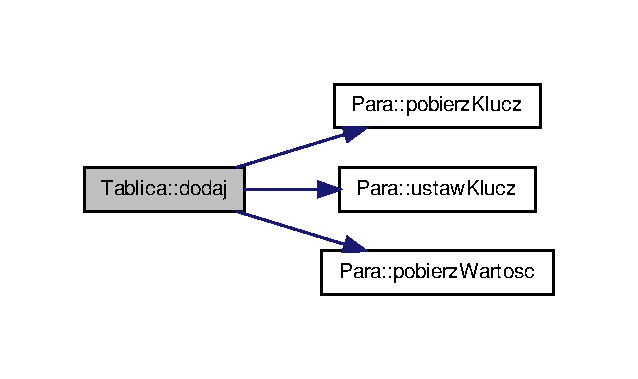
\includegraphics[width=306pt]{class_tablica_aebb17d3366e37c8b4852df08eae2a1de_cgraph}
\end{center}
\end{figure}




\-Oto graf wywoływań tej funkcji\-:\nopagebreak
\begin{figure}[H]
\begin{center}
\leavevmode
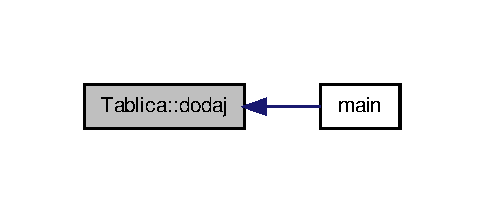
\includegraphics[width=232pt]{class_tablica_aebb17d3366e37c8b4852df08eae2a1de_icgraph}
\end{center}
\end{figure}


\hypertarget{class_tablica_a8fd66d75553eb44aa043f917fd9317dc}{\index{\-Tablica@{\-Tablica}!haszstring@{haszstring}}
\index{haszstring@{haszstring}!Tablica@{\-Tablica}}
\subsubsection[{haszstring}]{\setlength{\rightskip}{0pt plus 5cm}template$<$typename K , typename W $>$ int {\bf \-Tablica}$<$ \-K, \-W $>$\-::{\bf haszstring} (
\begin{DoxyParamCaption}
\item[{\-K}]{key}
\end{DoxyParamCaption}
)\hspace{0.3cm}{\ttfamily  \mbox{[}private\mbox{]}}}}\label{class_tablica_a8fd66d75553eb44aa043f917fd9317dc}


\-Funkcja haszujaca dla obiektow typu string. 

\hypertarget{class_tablica_a7f5a2d2ebe594ec98dd38dfbbb83497d}{\index{\-Tablica@{\-Tablica}!operator\mbox{[}$\,$\mbox{]}@{operator[]}}
\index{operator\mbox{[}$\,$\mbox{]}@{operator[]}!Tablica@{\-Tablica}}
\subsubsection[{operator[]}]{\setlength{\rightskip}{0pt plus 5cm}template$<$typename K , typename W $>$ \-W \& {\bf \-Tablica}$<$ \-K, \-W $>$\-::operator\mbox{[}$\,$\mbox{]} (
\begin{DoxyParamCaption}
\item[{\-K}]{klucz}
\end{DoxyParamCaption}
)}}\label{class_tablica_a7f5a2d2ebe594ec98dd38dfbbb83497d}


\-Przeciazenie operatora indeksujacego. 

\begin{DoxyReturn}{\-Zwraca}
\-Zwraca wartosc. 
\end{DoxyReturn}


\-Oto graf wywołań dla tej funkcji\-:\nopagebreak
\begin{figure}[H]
\begin{center}
\leavevmode
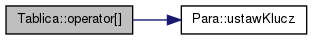
\includegraphics[width=306pt]{class_tablica_a7f5a2d2ebe594ec98dd38dfbbb83497d_cgraph}
\end{center}
\end{figure}


\hypertarget{class_tablica_a6de46e3062f16d78c4cb2cf18c9b0de1}{\index{\-Tablica@{\-Tablica}!pobierz\-Wartosc@{pobierz\-Wartosc}}
\index{pobierz\-Wartosc@{pobierz\-Wartosc}!Tablica@{\-Tablica}}
\subsubsection[{pobierz\-Wartosc}]{\setlength{\rightskip}{0pt plus 5cm}template$<$typename K , typename W $>$ \-W {\bf \-Tablica}$<$ \-K, \-W $>$\-::{\bf pobierz\-Wartosc} (
\begin{DoxyParamCaption}
\item[{\-K}]{klucz}
\end{DoxyParamCaption}
)}}\label{class_tablica_a6de46e3062f16d78c4cb2cf18c9b0de1}


\-Funkcja pobierz\-Wartosc. 

\begin{DoxyReturn}{\-Zwraca}
\-Zwraca wartosc przypisana do danego klucza. 
\end{DoxyReturn}


\-Oto graf wywoływań tej funkcji\-:\nopagebreak
\begin{figure}[H]
\begin{center}
\leavevmode
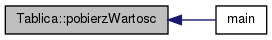
\includegraphics[width=276pt]{class_tablica_a6de46e3062f16d78c4cb2cf18c9b0de1_icgraph}
\end{center}
\end{figure}


\hypertarget{class_tablica_aabc40f316cf398a07e3035b1c4adc256}{\index{\-Tablica@{\-Tablica}!size@{size}}
\index{size@{size}!Tablica@{\-Tablica}}
\subsubsection[{size}]{\setlength{\rightskip}{0pt plus 5cm}template$<$typename \-K, typename \-W$>$ int {\bf \-Tablica}$<$ \-K, \-W $>$\-::{\bf size} (
\begin{DoxyParamCaption}
{}
\end{DoxyParamCaption}
)\hspace{0.3cm}{\ttfamily  \mbox{[}inline\mbox{]}}}}\label{class_tablica_aabc40f316cf398a07e3035b1c4adc256}


\-Podaje liczbe elementow w tablicy. 

\begin{DoxyReturn}{\-Zwraca}
zwraca liczbe elementow w tablicy. 
\end{DoxyReturn}
\hypertarget{class_tablica_a061a219dd25c6696940f40226d99a99d}{\index{\-Tablica@{\-Tablica}!usun@{usun}}
\index{usun@{usun}!Tablica@{\-Tablica}}
\subsubsection[{usun}]{\setlength{\rightskip}{0pt plus 5cm}template$<$typename K , typename W $>$ void {\bf \-Tablica}$<$ \-K, \-W $>$\-::{\bf usun} (
\begin{DoxyParamCaption}
\item[{\-K}]{klucz}
\end{DoxyParamCaption}
)}}\label{class_tablica_a061a219dd25c6696940f40226d99a99d}


\-Funkcja usun. \-Usuwa krotke o podanym kluczu. 



\-Oto graf wywoływań tej funkcji\-:\nopagebreak
\begin{figure}[H]
\begin{center}
\leavevmode
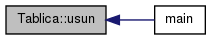
\includegraphics[width=230pt]{class_tablica_a061a219dd25c6696940f40226d99a99d_icgraph}
\end{center}
\end{figure}




\subsection{\-Dokumentacja atrybutów składowych}
\hypertarget{class_tablica_a603b571fcc0d29b757bfd5fe27d0fadc}{\index{\-Tablica@{\-Tablica}!liczba\-Elementow@{liczba\-Elementow}}
\index{liczba\-Elementow@{liczba\-Elementow}!Tablica@{\-Tablica}}
\subsubsection[{liczba\-Elementow}]{\setlength{\rightskip}{0pt plus 5cm}template$<$typename \-K, typename \-W$>$ int {\bf \-Tablica}$<$ \-K, \-W $>$\-::{\bf liczba\-Elementow}\hspace{0.3cm}{\ttfamily  \mbox{[}private\mbox{]}}}}\label{class_tablica_a603b571fcc0d29b757bfd5fe27d0fadc}


\-Obecna liczba elementow w tablicy. 

\hypertarget{class_tablica_a40b3c86ceb2ec860b9d19ce0e866b406}{\index{\-Tablica@{\-Tablica}!rozmiar@{rozmiar}}
\index{rozmiar@{rozmiar}!Tablica@{\-Tablica}}
\subsubsection[{rozmiar}]{\setlength{\rightskip}{0pt plus 5cm}template$<$typename \-K, typename \-W$>$ int {\bf \-Tablica}$<$ \-K, \-W $>$\-::{\bf rozmiar}\hspace{0.3cm}{\ttfamily  \mbox{[}private\mbox{]}}}}\label{class_tablica_a40b3c86ceb2ec860b9d19ce0e866b406}


\-Maksymalna liczba elementow w tablicy. 

\hypertarget{class_tablica_a0d6b03ac0a2b996d4096038ef9315e9a}{\index{\-Tablica@{\-Tablica}!tablica@{tablica}}
\index{tablica@{tablica}!Tablica@{\-Tablica}}
\subsubsection[{tablica}]{\setlength{\rightskip}{0pt plus 5cm}template$<$typename \-K, typename \-W$>$ {\bf \-Para}$<$\-K,\-W$>$$\ast$$\ast$ {\bf \-Tablica}$<$ \-K, \-W $>$\-::{\bf tablica}\hspace{0.3cm}{\ttfamily  \mbox{[}private\mbox{]}}}}\label{class_tablica_a0d6b03ac0a2b996d4096038ef9315e9a}


\hyperlink{class_tablica}{\-Tablica} par. 



\-Dokumentacja dla tej klasy została wygenerowana z pliku\-:\begin{DoxyCompactItemize}
\item 
\hyperlink{_tablica_8h}{\-Tablica.\-h}\end{DoxyCompactItemize}

\chapter{\-Dokumentacja plików}
\hypertarget{main_8cpp}{\section{\-Dokumentacja pliku /home/martyna/\-Pulpit/calka/prj/main.cpp}
\label{main_8cpp}\index{/home/martyna/\-Pulpit/calka/prj/main.\-cpp@{/home/martyna/\-Pulpit/calka/prj/main.\-cpp}}
}


\-Plik zawiera glowna funkcje programu.  


{\ttfamily \#include $<$iostream$>$}\*
{\ttfamily \#include \char`\"{}integral.\-h\char`\"{}}\*
\-Wykres zależności załączania dla main.\-cpp\-:\nopagebreak
\begin{figure}[H]
\begin{center}
\leavevmode
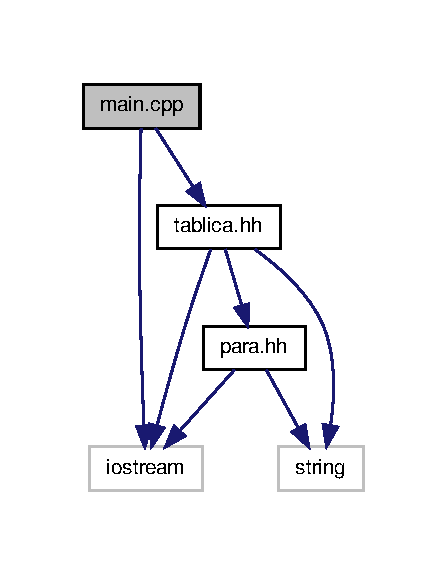
\includegraphics[width=272pt]{main_8cpp__incl}
\end{center}
\end{figure}
\subsection*{\-Funkcje}
\begin{DoxyCompactItemize}
\item 
double \hyperlink{main_8cpp_a80abd7257657e8a5b78f917731d87ba5}{\-F} (double x)
\item 
int \hyperlink{main_8cpp_ae66f6b31b5ad750f1fe042a706a4e3d4}{main} ()
\end{DoxyCompactItemize}


\subsection{\-Opis szczegółowy}
\-Plik zawiera glowna funkcje programu. 

\-Definicja w pliku \hyperlink{main_8cpp_source}{main.\-cpp}.



\subsection{\-Dokumentacja funkcji}
\hypertarget{main_8cpp_a80abd7257657e8a5b78f917731d87ba5}{\index{main.\-cpp@{main.\-cpp}!\-F@{\-F}}
\index{\-F@{\-F}!main.cpp@{main.\-cpp}}
\subsubsection[{\-F}]{\setlength{\rightskip}{0pt plus 5cm}double {\bf \-F} (
\begin{DoxyParamCaption}
\item[{double}]{x}
\end{DoxyParamCaption}
)}}\label{main_8cpp_a80abd7257657e8a5b78f917731d87ba5}


\-Definicja w linii 11 pliku main.\-cpp.



\-Oto graf wywoływań tej funkcji\-:\nopagebreak
\begin{figure}[H]
\begin{center}
\leavevmode
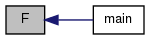
\includegraphics[width=184pt]{main_8cpp_a80abd7257657e8a5b78f917731d87ba5_icgraph}
\end{center}
\end{figure}


\hypertarget{main_8cpp_ae66f6b31b5ad750f1fe042a706a4e3d4}{\index{main.\-cpp@{main.\-cpp}!main@{main}}
\index{main@{main}!main.cpp@{main.\-cpp}}
\subsubsection[{main}]{\setlength{\rightskip}{0pt plus 5cm}int {\bf main} (
\begin{DoxyParamCaption}
{}
\end{DoxyParamCaption}
)}}\label{main_8cpp_ae66f6b31b5ad750f1fe042a706a4e3d4}


\-Definicja w linii 15 pliku main.\-cpp.



\-Oto graf wywołań dla tej funkcji\-:\nopagebreak
\begin{figure}[H]
\begin{center}
\leavevmode
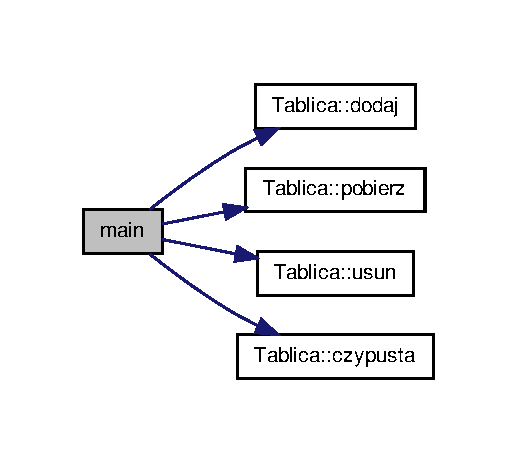
\includegraphics[width=350pt]{main_8cpp_ae66f6b31b5ad750f1fe042a706a4e3d4_cgraph}
\end{center}
\end{figure}



\hypertarget{para_8hh}{\section{\-Dokumentacja pliku para.\-hh}
\label{para_8hh}\index{para.\-hh@{para.\-hh}}
}


\-Definicja szablonu klasy \-Para \-Plik zawiera definicję szablonu klasy \-Para.  


{\ttfamily \#include $<$string$>$}\*
{\ttfamily \#include $<$iostream$>$}\*
\-Wykres zależności załączania dla para.\-hh\-:\nopagebreak
\begin{figure}[H]
\begin{center}
\leavevmode
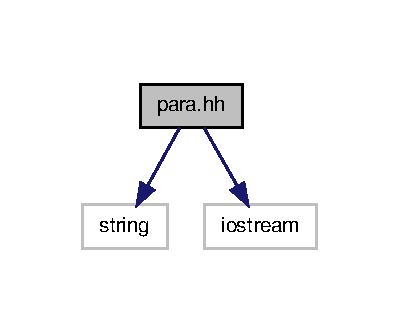
\includegraphics[width=192pt]{para_8hh__incl}
\end{center}
\end{figure}
\-Ten wykres pokazuje, które pliki bezpośrednio lub pośrednio załączają ten plik\-:\nopagebreak
\begin{figure}[H]
\begin{center}
\leavevmode
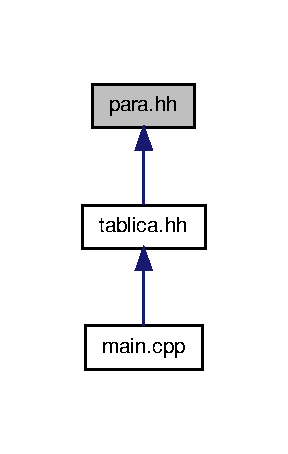
\includegraphics[width=138pt]{para_8hh__dep__incl}
\end{center}
\end{figure}
\subsection*{\-Komponenty}
\begin{DoxyCompactItemize}
\item 
class \hyperlink{classpara}{para$<$ K, V $>$}
\begin{DoxyCompactList}\small\item\em \-Modeluje pojęcie para. \-Jej atrybutem są pola zawierające klucz i wartość. \end{DoxyCompactList}\end{DoxyCompactItemize}


\subsection{\-Opis szczegółowy}


\-Definicja w pliku \hyperlink{para_8hh_source}{para.\-hh}.


\hypertarget{tablica_8hh}{\section{\-Dokumentacja pliku tablica.\-hh}
\label{tablica_8hh}\index{tablica.\-hh@{tablica.\-hh}}
}


\-Definicja szablonu klasy \-Tablica(\-Tablica asocjacyjna)  


{\ttfamily \#include \char`\"{}para.\-hh\char`\"{}}\*
{\ttfamily \#include $<$iostream$>$}\*
{\ttfamily \#include $<$string$>$}\*
\-Wykres zależności załączania dla tablica.\-hh\-:\nopagebreak
\begin{figure}[H]
\begin{center}
\leavevmode
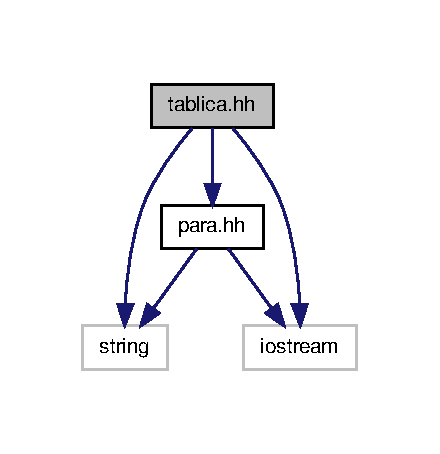
\includegraphics[width=211pt]{tablica_8hh__incl}
\end{center}
\end{figure}
\-Ten wykres pokazuje, które pliki bezpośrednio lub pośrednio załączają ten plik\-:\nopagebreak
\begin{figure}[H]
\begin{center}
\leavevmode
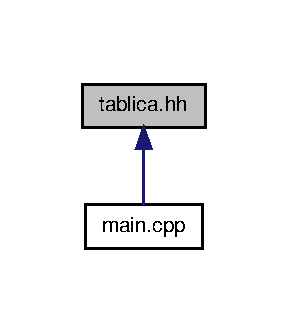
\includegraphics[width=138pt]{tablica_8hh__dep__incl}
\end{center}
\end{figure}
\subsection*{\-Komponenty}
\begin{DoxyCompactItemize}
\item 
class \hyperlink{class_tablica}{\-Tablica$<$ K, V $>$}
\begin{DoxyCompactList}\small\item\em \-Modeluje pojęcie \hyperlink{class_tablica}{\-Tablica}. \-Klasa modeluje pojęcie \hyperlink{class_tablica}{\-Tablica} asocjacyjna . \-Jej atrybutem są pola\-: klucz i wartość. \end{DoxyCompactList}\end{DoxyCompactItemize}
\subsection*{\-Definicje}
\begin{DoxyCompactItemize}
\item 
\#define \hyperlink{tablica_8hh_aa50aa866c5823769bb02e986d29a0589}{\-R\-O\-Z\-M\-I\-A\-R}~100
\end{DoxyCompactItemize}


\subsection{\-Opis szczegółowy}
\-Plik zawiera definicję szablonu klasy \-Tablica.\-Jest to klasa główna , która wykorzystuje klasę para. 

\-Definicja w pliku \hyperlink{tablica_8hh_source}{tablica.\-hh}.



\subsection{\-Dokumentacja definicji}
\hypertarget{tablica_8hh_aa50aa866c5823769bb02e986d29a0589}{\index{tablica.\-hh@{tablica.\-hh}!\-R\-O\-Z\-M\-I\-A\-R@{\-R\-O\-Z\-M\-I\-A\-R}}
\index{\-R\-O\-Z\-M\-I\-A\-R@{\-R\-O\-Z\-M\-I\-A\-R}!tablica.hh@{tablica.\-hh}}
\subsubsection[{\-R\-O\-Z\-M\-I\-A\-R}]{\setlength{\rightskip}{0pt plus 5cm}\#define {\bf \-R\-O\-Z\-M\-I\-A\-R}~100}}\label{tablica_8hh_aa50aa866c5823769bb02e986d29a0589}


\-Definicja w linii 10 pliku tablica.\-hh.


\printindex
\end{document}
